% % % % % % % % % % % % % % % % % % % % % % % % % % % % % % % % % % % % % % % % % % % %
%                                                                                     %
% Short Sectioned Assignment LaTeX Template Version 1.0 (5/5/12)                      %
% This template has been downloaded from: http://www.LaTeXTemplates.com               %
%                                                                                     %
% Original author:  Frits Wenneker (http://www.howtotex.com)                          %
%                                                                                     %
% Modified by: Fco Javier Sueza Rodríguez (fcosueza@disroot.org)                      %
%                                                                                     %
% Changes:                                                                            %
%	    - Custom Chapters, Sections and Subsections (titlesec package)                %
%           - Document type scrbook (oneside)                                         %
%           - Use babel-lang-spanish package and marvosym                             %
%           - Use hyperref, enumitem, tcolorbox and glossaries packages               %
%           - Use Time New Roman (mathptmx), Helvetic and Courier fonts               %
%                                                                                     %
% License: CC BY-NC-SA 3.0 (http://creativecommons.org/licenses/by-nc-sa/3.0/)        %
%                                                                                     %
% % % % % % % % % % % % % % % % % % % % % % % % % % % % % % % % % % % % % % % % % % % %

%-----------------------------------------------%
%	              Packages                  %
%-----------------------------------------------%

\documentclass[paper=a4, fontsize=11pt, oneside]{scrbook}

% ---- Text Input/Output ----- %

\usepackage[T1]{fontenc}
\usepackage[utf8]{inputenc}
\usepackage{mathptmx}
\usepackage[scaled=.92]{helvet}
\usepackage{courier}
\usepackage[indent=12pt]{parskip}

\usepackage{geometry}
\geometry{verbose,tmargin=3cm,bmargin=3cm,lmargin=2.6cm,rmargin=2.6cm}

% ---- Language ----- %

\usepackage[spanish]{babel}
\usepackage{marvosym}

% ---- Another packages ---- %

\usepackage{amsmath,amsfonts,amsthm}
\usepackage{graphics,graphicx}
\usepackage{titlesec}
\usepackage{fancyhdr}
\usepackage{tcolorbox}
\usepackage{hyperref}
\usepackage{enumitem}
\usepackage[automake]{glossaries}

%--------------------------------------------------------------------%
%                      Customizing Document                          %
%--------------------------------------------------------------------%


% ----------- Custom Chapters, Sections and Subsections -------------- %

\titleformat{\chapter}[display]
			{\bfseries\Huge}
			{Tema \ \thechapter} {0.5ex}
			{\vspace{1ex}\centering}

\titleformat{\section}[hang]
			{\bfseries\Large}
			{\thesection}{0.5em}{}

\titleformat{\subsection}[hang]
			{\bfseries\large}
			{\thesubsection}{0.5em}{}

\titleformat{\subsubsection}[hang]
			{\bfseries\large}
			{\thesubsubsection}{0.5em}{}

\hypersetup{
    colorlinks=true,
    linkcolor=black,
    urlcolor=magenta
}

% ------------------- Custom heaaders and footers ------------------- %

\pagestyle{fancyplain}

\fancyhead[]{}
\fancyfoot[L]{}
\fancyfoot[C]{}
\fancyfoot[R]{\thepage}

\renewcommand{\headrulewidth}{0pt} % Remove header underlines
\renewcommand{\footrulewidth}{0pt} % Remove footer underlines

\setlength{\headheight}{13.6pt} % Customize the height of the header

% --------- Numbering equations, figures and tables ----------------- %

\numberwithin{equation}{section} % Number equations within sections
\numberwithin{figure}{section} % Number figures within sections
\numberwithin{table}{section} % Number tables within sections

% ------------------------ New Commands ----------------------------- %

\newcommand{\horrule}[1]{\rule{\linewidth}{#1}} % Create horizontal rule command


%----------------------------------------------------------------------------------------
%	TÍTULO Y DATOS DEL ALUMNO
%----------------------------------------------------------------------------------------

\title{
\normalfont \normalsize
\textsc{{\bfseries Curso 2022-2023} \\ Ciclo Superior de Desarrollo de Aplicaciones Web \\ IES Aguadulce} \\ [25pt]
\horrule{0.5pt} \\[0.4cm]
\huge Entornos de Desarrollo \\
\horrule{0.5pt} \\[0.4cm]
}

\author{Francisco Javier Sueza Rodríguez}
\date{\normalsize\today}

%----------------------------------------------------------------------------------------
%                                     DOCUMENTO
%----------------------------------------------------------------------------------------

\makeglossaries
\loadglsentries{glossary.tex}

\begin{document}

\maketitle

\newpage

\tableofcontents

\listoffigures

%\listoftables

\newpage

\chapter{Desarrollo de Software}
En esta unidad vamos a realizar una introducción al concepto de software, así como a los diferentes tipos de software que podemos encontrar y al proceso de desarrollo de éste. También hablaremos de los lenguajes de programación, en que consiste y que características tiene. Por último, veremos que son los entornos de desarrollo, cuales su función y su evolución histórica.

\section{Software y Tipos de Software}
Un ordenador se compone de dos partes bien diferenciadas, el {\bfseries hardware} y el {\bfseries software}.

El {\bfseries hardware}, {\bfseries equipo} o {\bfseries soporte físico} en informática se refiere a las partes físicas, tangibles de un sistema informático, sus componentes eléctricos, electrónicos y electromecánicos. Los cables, así como los muebles o cajas de todo tipo también se incluyen dentro de esta categoría. \cite{wiki01}

Por otro lado, el {\bfseries software} es el conjunto de componentes lógicos que hace posible la realización de tareas específicas \cite{wiki02}. Dicho de otra forma, es el conjunto de programas informáticos que actúa sobre el hardware para ejecutar lo que el usuario desee.

Según su funcionalidad, podemos diferencias tres tipos principales de software:

\begin{itemize}
    \item {\bfseries Sistema Operativo}: conjunto de programas de un sistema informático que gestiona los recursos hardware y provee servicios a las aplicaciones informáticas para su funcionamiento. Ejemplos de sistemas operativos son: \gls{Microsoft Windows}, \gls{Linux}, \gls{macOS}...
    \item {\bfseries Software de Programación}: conjunto de herramientas y utilidades que permiten a los programadores desarrollar programas informáticos.
    \item {\bfseries Aplicaciones Informáticas}: programas o conjunto de programas que tienen una aplicación concreta. Algunos ejemplos de aplicaciones informáticas son los procesadores de texto, reproductores multimedia, juegos...
\end{itemize}

Aunque estos son los tipos principales de software, podemos ampliar esta clasificación incluyendo los siguientes tipos, los cuales son, en mayor medida, subdivisiones de las aplicaciones informáticas \cite{tipos}:

\begin{itemize}
    \item {\bfseries Software de Tiempo Real}: son aquellos programas que se usan en sistemas de tiempo real y que reaccionan con el entorno físico respondiendo a los estímulos del éste en un tiempo limitado. Ejemplos de este software son los sistemas de control de procesos, aplicaciones de robótica,..
    \item {\bfseries Software de Gestión}: son programas que utilizan grandes cantidades de información almacenadas en bases de datos para ayudar a la administración y toma de decisiones. Un ejemplo de estos sistemas son los {\bfseries \gls{ERP}}.
    \item {\bfseries Software Científico o de Ingeniería}: software que se encarga de realizar complejos cálculos numéricos de todo tipo, siendo la corrección y exactitud en estos cálculos uno de los requisitos básicos. También incluye los sistemas de diseño, ingeniería y fabricación asistida por ordenador (CAD, CAE y CAM), simuladores gráficos,..
    \item {\bfseries Software Empotrado}: software que por norma general va instalado en memorias ROM y sirve para controlar productos y sistemas de los mercados industriales. Se aplica a todo tipo de productos como neveras, reproductores de vídeo, misiles, sistemas de control de automóviles,...
    \item {\bfseries Software de Inteligencia Artificial}: software que basándose en el uso de lenguajes declarativos, sistemas expertos y redes neuronales, para simular comportamientos humanos como el aprendizaje, razonamiento y la resolución de problemas para la realización de forma fiable y rápida operaciones que para el ser humano son tediosas o incluso inabordables. Ejemplos de estas aplicaciones son las aplicaciones de \textit{machine learning}, chatbots,...
\end{itemize}

En este tema, nos centraremos en las {\bfseries aplicaciones informáticas}, como se desarrollan y cuales son las fases de este desarrollo. También veremos el {\bfseries ciclo de vida de una aplicación informática} y los diferentes tipos de {\bfseries lenguajes de programación} y sus características.

\section{Relación Hardware-Software}
Como hemos comentado en el punto anterior, un sistemas informático se compone de hardware y software. Existe una relación indisoluble entre estos dos componentes ya que se necesita que estén instalados y configurados correctamente para que el ordenador funcione.

El primer modelo de arquitectura de hardware con programa almacenado fue propuesto por {\bfseries John Von Neumman} en 1946. A continuación se muestra una imagen con las diferentes partes de esta arquitectura:

\begin{figure}[h]
    \centering
    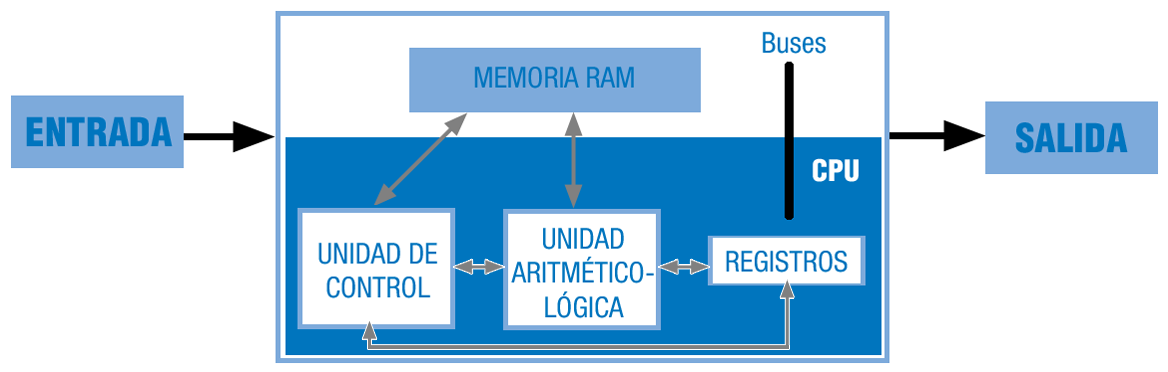
\includegraphics[scale=0.38]{von-neumman.png}
    \caption{Arquitectura John Von Neuman}
\end{figure}

Esta relación software-hardware la podemos analizar desde dos puntos de vista diferentes:

\begin{enumerate}[label={\alph*}]
    \item {\bfseries Desde el punto de vista del sistema operativo}: el sistema operativo es el encargado de coordinar
    el funcionamiento del ordenador, actuando entre este y las aplicaciones que están corriendo en ese momento, gestionando los diferentes recursos hardware que requieren estas aplicaciones (CPU, RAM, interrupciones, dispositivos de E/S..).
    \item {\bfseries Desde el punto de vista de las aplicaciones}: una aplicación solo es un conjunto de programas  escritos en algún lenguaje de programación. Hay multitud de lenguajes de programación, con la característica de que todos están escritos en un idioma que el ser humano puede entender. El hardware por otro lado solo es capaz de interpretar señales eléctricas que se traducen en secuencias de 0 y 1 (código binario). Para que estás aplicaciones puedan ejecutarse en el hardware debe darse un proceso de "traducción" que veremos mas adelante.
\end{enumerate}

\section{Desarrollo de Software}
Entendemos por {\bfseries \gls{Desarrollo de Software}} todo el proceso desde que se concibe la idea hasta que el programa está implementado y funcionando en el ordenador. Aunque en principio pueda parecer una tarea simple, consta de una series de pasos de obligado cumplimiento, pues solo así podemos garantizar que las aplicaciones creadas son eficientes, seguras, fiables y responden a las necesidades de los usuarios finales.

Como veremos más adelante en la unidad, esta serie de pasos se le suele denominar {\bfseries Etapas} en el desarrollo de software. Según el orden y la forma en la que se llevan a cabo estas etapas hablaremos de diferentes ciclos de vida del software. \\

\begin{figure}[h]
    \centering
    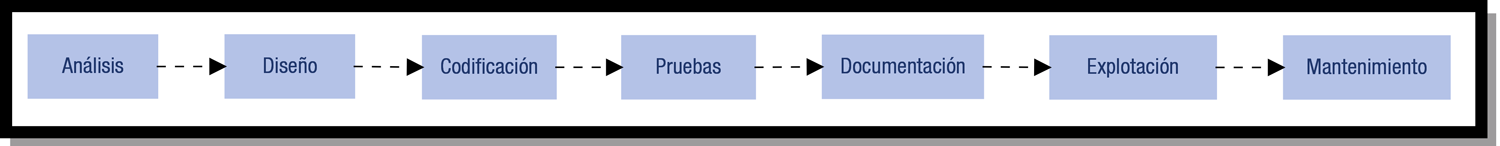
\includegraphics[scale=0.8]{etapas-desarrollo.png}
    \caption{Etapas del Desarrollo de Software}
\end{figure}

Cabe destacar que la construcción de software es un proceso muy complejo y que requiere de una gran coordinación y disciplina del grupo de trabajo que lo desarrolle.

\subsection{Ciclos de Vida del Software}
Ya hemos visto que para crear software debemos seguir un número de pasos conocidos como ciclo de vida del software. Más adelante en esta unidad veremos en que consiste cada paso mas detalladamente. Por ahora, vamos a centrarnos en ver los diferentes ciclos de vida del software que existen atendiendo a como se desarrollan dichos pasos.

Aunque podemos encontrar diferentes clasificaciones sobre los distintos tipos de ciclos de vida del software los mas conocidos y utilizados son los siguientes:

\begin{enumerate}
    \item {\bfseries Modelo en Cascada}: es el modelo de vida clásico del software. Actualmente es prácticamente imposible de utilizar, salvo para desarrollos muy pequeños, ya que es necesario conocer todos los requisitos con antelación y las etapas pasan de una a otra sin retorno, presuponiendo que no ha habido errores en la etapa anterior.
    \item {\bfseries Modelo en Cascada con Realimentación}: es uno de los modelos más utilizados. Proviene del modelo anterior, pero se introduce una realimentación entre etapas, permitiendo que podamos volver hacia atrás en cualquier momento para corregir, depurar o modificar algún aspecto. Es el modelo perfecto si el proyecto es es rígido (pocos cambios y poco evolutivo) y los requisitos están claros. No obstante, si se prevén muchos cambios durante el desarrollo no es el modelo más idóneo.
    \item {\bfseries Modelos Evolutivos}: son los modelos más modernos y tienen en cuenta el aspecto cambiante y evolutivo del software. Dentro de este modulo podemos encontrar dos variantes:
    \begin{enumerate}[label*=\arabic*.]
        \item {\bfseries Modelo Iterativo Incremental}: ésta basado en el modelo en cascada con realimentación, donde las fases se repiten y refinan, propagando su mejora a las fases siguientes. El proyecto se realiza en pequeñas porciones ({\bfseries incrementa}) en sucesivas iteraciones ({\bfseries sprints}) al final de las cuales se ve lo que se ha desarrollado, pudiendo hacer correcciones o modificaciones antes de la siguiente iteración o incluso añadir nuevos requerimientos ({\bfseries adaptativo}). Cada sprint debe proporcional un resultado completo preparado para entregárselo al clientes.
        \item {\bfseries Modelo en Espiral}: es una combinación del modelo anterior con el modelo en cascada. En éste, el software se va construyendo repetidamente en forma de versiones que son cada vez mejores, debido a que se va incrementando la funcionalidad. Es un modelo muy complejo.
    \end{enumerate}
\end{enumerate}

En la actualidad, la {metodologías de desarrollo ágil}, enmarcadas dentro de los modelos evolutivos, están en auge, y metodologías como {\bfseries \href{https://es.wikipedia.org/wiki/Scrum_(desarrollo_de_software)}{Scrum}}, {\bfseries \href{https://es.wikipedia.org/wiki/Desarrollo_guiado_por_pruebas}{TDD}} o {\bfseries \href{https://es.wikipedia.org/wiki/Desarrollo_guiado_por_comportamiento}{BDD}}, así como metodologías híbridas basadas en estas, se están convirtiendo en el estándar de la industria. \cite{batool01}

\subsection{Herramientas de Apoyo al Desarrollo De Software}







% Glossary

\glsaddall
\printglossaries

% Bibliography

\newpage
\addcontentsline{toc}{chapter}{Bibliografía}
\bibliography{citas}
\bibliographystyle{unsrt}

\end{document}